\documentclass[compress,red]{beamer}
\usepackage{etex}
\mode<presentation>

\usetheme{Warsaw}

\setbeamertemplate{navigation symbols}{}
\setbeamertemplate{headline}{}

%\setbeameroption{show notes}
%\setbeameroption{show only notes}
\setbeameroption{hide notes}

%\hypersetup{pdfpagemode=FullScreen} % makes your presentation go automatically to full screen
%\useoutertheme[subsection=false]{smoothbars}
\useoutertheme{shadow}

% include packages
\usepackage{subfigure}
\usepackage{textcomp}
\usepackage{multicol}
\usepackage{amsmath}
\usepackage{epsfig}
\usepackage{graphicx}
\usepackage[all,knot]{xy}
\xyoption{arc}
\usepackage{url}
\usepackage{multimedia}
\usepackage{hyperref}
\usepackage{helvet}
\usepackage[english]{babel}
\usepackage[utf8]{inputenc}
\usepackage{multirow}
\usepackage{verbatim}
%\usepackage{geometry}
%\geometry{verbose,letterpaper}
%\usepackage{movie15}
%\usepackage{hyperref}
\usepackage{pgfpages}
\usepackage{setspace}


\graphicspath{{../pictures/}}

\titlegraphic{\scalebox{4}{
    \includegraphics[height=0.5cm]{ohwr_logo.eps}
  }
}


\title[{\makebox[.45\paperwidth]{F*WATCH\hfill%
       \insertframenumber/\inserttotalframenumber}}]{F*WATCH, making a watch differently!}


\author
{Federico Vaga, Matthieu Cattin}

\date
{FOSDEM, Brussels, 31 January 2015}

\begin{document}

\begin{frame}
  \titlepage
\end{frame}


%#####################################################################
%############ SECTION ################################################
\section{Introduction}

\subsection*{} % dummy subsection to display dots

%------------ FRAME --------------------------------------------------
\begin{frame}{What is it?}
  \begin{center}
      \alt<2> {
        \includegraphics[height=7.5cm]{fwatch-full-side-red.eps}
      }{
        \includegraphics[height=7.5cm]{fwatch-full-side-black-qmark.eps}
      }
  \end{center}
\end{frame}

%------------ FRAME --------------------------------------------------
\begin{frame}{Why a watch?}
  \Large
  \begin{center}
    Retirement gift for a timing Hacker \\
  \end{center}
  \vskip 1cm

  \textbf{Gift Requirement}
  \vskip 7mm
  \begin{enumerate}
  \item customization of the gift
    %\vskip mm
  \item hackable gift
    %\vskip 7mm
  \item free/open source
    %\vskip 7mm
  \item use only FOSS tools
  \end{enumerate}

\end{frame}

%------------ FRAME --------------------------------------------------
\begin{frame}{Development organization}
  \begin{center}
    \includegraphics[height=7cm]{fwatch-team.eps}
  \end{center}

\end{frame}


%#####################################################################
%############ SECTION ################################################
\section{The design}

%------------ FRAME --------------------------------------------------
\begin{frame}{The design}

  Components selection criteria
  \vskip 5mm

  \begin{itemize}
  \item Low power consumption
    \vskip 5mm
  \item Available in small quantity from main suppliers
    \vskip 5mm
  \item Small size (footprint)
  \end{itemize}

\end{frame}

%------------ FRAME --------------------------------------------------
\begin{frame}{Components selection}

  \begin{columns}[T] % align columns
    \begin{column}{.48\textwidth}

      Micro-controller (EFM32)
      \vskip 6mm
      \begin{itemize}
      \item Silicon Labs
      \item 32-bit Cortex-M3
      \item 1MB flash
      \item 128kB RAM
      \item 1.1uA deep sleep
      \end{itemize}

    \end{column}
    \hfill%
    \begin{column}{.48\textwidth}
      \includegraphics[height=5cm]{mcu_efm32.eps}
    \end{column}%
  \end{columns}

\end{frame}

%------------ FRAME --------------------------------------------------
\begin{frame}{Components selection}

  \begin{columns}[T] % align columns
    \begin{column}{.48\textwidth}

      GPS module
      \vskip 6mm
      \begin{itemize}
      \item Antenova
      \item 13 x 9.5 x 1.8mm
      \item Integrated antenna
      \end{itemize}

    \end{column}
    \hfill%
    \begin{column}{.48\textwidth}
      \includegraphics[height=5cm]{M10478-A1.eps}
    \end{column}%
  \end{columns}

\end{frame}

%------------ FRAME --------------------------------------------------
\begin{frame}{Components selection}

  \begin{columns}[T] % align columns
    \begin{column}{.48\textwidth}

      Altimeter module \\
      (pressure sensor)
      \vskip 6mm
      \begin{itemize}
      \item Measurement Specialties
      \item 6.4 x 4 x 2.8mm
      \item Water-resistant
      \item Includes a thermometer
      \end{itemize}

    \end{column}
    \hfill%
    \begin{column}{.48\textwidth}
      \includegraphics[height=4.5cm]{MS5806-02BA52-51.eps}
    \end{column}%
  \end{columns}

\end{frame}

%------------ FRAME --------------------------------------------------
\begin{frame}{Components selection}

  \begin{columns}[T] % align columns
    \begin{column}{.48\textwidth}

      Memory LCD display
      \vskip 6mm
      \begin{itemize}
      \item Sharp
      \item 128 x 128 pixels
      \item 1.28 inches
      \item Ultra low current
      \end{itemize}

    \end{column}
    \hfill%
    \begin{column}{.48\textwidth}
      \includegraphics[height=4.5cm]{LCD.eps}
    \end{column}%
  \end{columns}

\end{frame}

%------------ FRAME --------------------------------------------------
\begin{frame}{Components selection}

  \begin{columns}[T] % align columns
    \begin{column}{.48\textwidth}

      Battery
      \vskip 6mm
      \begin{itemize}
      \item Adafruit
      \item Li-ion 500mAh
      \item Big capacity
      \item Lightweight
      \item Rechargeable
      \end{itemize}

    \end{column}
    \hfill%
    \begin{column}{.48\textwidth}
      \includegraphics[height=4.5cm]{battery.eps}
    \end{column}%
  \end{columns}

\end{frame}

%------------ FRAME --------------------------------------------------
\begin{frame}{Components selection}

  Other features
  \begin{itemize}
  \item 3-axis accelerometer + compass
  \item Ambient light sensor
  \item micro-SD card slot
  \item Battery charger + fuel gauge
  \item micro-USB connector
  \item Buzzer
  \item Vibrating motor
  \end{itemize}

  \vskip 5mm
  Foreseen improvements
  \begin{itemize}
  \item Bluetooth LE
  \item Low noise amplifier for the GPS antenna
  \item Power management
  \end{itemize}

\end{frame}

%------------ FRAME --------------------------------------------------
\begin{frame}{PCB design}

  \begin{center}
    \includegraphics[height=1cm]{kicad_logo.eps}
  \end{center}

  \begin{itemize}
  \item CERN is contributing
  \item Developers in the team (help, bugfix, feedback)
  \item New features making routing easier (e.g push\&shove)
  \item Script to generate placement pdf
  \end{itemize}

  \vskip 6mm
  Interested in knowing more about KiCad developments?
  \begin{itemize}
  \item Visit the EDA dev room (AW1.124) tomorrow
  \end{itemize}

\end{frame}

%------------ FRAME --------------------------------------------------
\begin{frame}{PCB design}

  Characteristics

  \begin{itemize}
  \item 4 x 4 cm
  \item 4 layers
  \item Components on both sides
  \item Licensed under CERN OHL v1.2
  \end{itemize}

  \begin{center}
    \includegraphics[height=4cm]{pcb_top.eps}~
    \includegraphics[height=4cm]{pcb_bottom.eps}
  \end{center}

\end{frame}

%------------ FRAME --------------------------------------------------
\begin{frame}{PCB assembly \& validation}

  Prototypes assembled by hand
  \vskip 5mm
  Fully working, except two minor bugs

  \begin{itemize}
  \item Error in a datasheet
  \item MCU interrupt scheme
  \end{itemize}

  $\rightarrow$ Fixed with few cuts and wires!

  \begin{center}
    \includegraphics[height=3cm]{pcb_mounted_bottom.eps}~
    \includegraphics[height=3cm]{pcb_mounted_top.eps}
  \end{center}

\end{frame}

%------------ FRAME --------------------------------------------------
\begin{frame}{Backlight}

  A long story...
  \vskip 8mm
  \begin{itemize}
  \item To read display in the dark
  \item No backlight available
  \end{itemize}

\end{frame}

%------------ FRAME --------------------------------------------------
\begin{frame}{Backlight}

  First try: LEDs + opaque Plexiglas

  \begin{center}
    \includegraphics[height=4.5cm]{bl_led_off.eps}~
    \pause
    \includegraphics[height=4.5cm]{bl_led_on.eps}
  \end{center}

  \textbf{Not good!}

\end{frame}

%------------ FRAME --------------------------------------------------
\begin{frame}{Backlight}

  Second try: Recycled smartphone backlight

  \begin{center}
    \includegraphics[height=4.5cm]{bl_smartphone_off.eps}~
    \pause
    \includegraphics[height=4.5cm]{bl_smartphone_on.eps}
  \end{center}

  \textbf{Better, but...}

\end{frame}

%------------ FRAME --------------------------------------------------
\begin{frame}{Backlight}

  Current try: Custom-made module

  $\rightarrow$ Low quantity, cheap ($<$ 5\$/pces)

  \begin{center}
    \includegraphics[height=4.5cm]{bl_custom_off.eps}~
    \pause
    \includegraphics[height=4.5cm]{bl_custom_on.eps}
  \end{center}

  \textbf{The solution}

\end{frame}

%------------ FRAME --------------------------------------------------
\begin{frame}{Mechanical design}

  CAD tool selection

  \begin{itemize}
  \item No mechanical engineer
  \item No experience in 3D design/printing
  \item Evaluate existing free CAD tools \\
    FreeCAD, OpenSCAD, Open CASCADE, ...
  \end{itemize}

  \pause
  Criteria

  \begin{itemize}
  \item Documentation, support
  \item User-friendliness, learning curve
  \end{itemize}

  \pause
  Decided to use \textbf{FreeCAD}

  \begin{center}
    \includegraphics[height=2cm]{freecad_logo.eps}
  \end{center}

\end{frame}

%------------ FRAME --------------------------------------------------
\begin{frame}{Mechanical design}

  Full of new challenges
  \vskip 5mm

  \begin{itemize}
  \item Learn FreeCAD from scratch
  \item Design a watch case
  \item 3D print it
  \end{itemize}

  \pause
  \vskip 9mm
  \begin{center}
    \Large It's time for a live demo!
  \end{center}

\end{frame}

%------------ FRAME --------------------------------------------------
\begin{frame}{3D model}

  \begin{center}
    \includegraphics[height=4.8cm]{case-design-model.eps}
  \end{center}

  Making of movie (6 hours summarised in 5 minutes)
  \url{http://www.ohwr.org/projects/f-watch/wiki/Movies}

\end{frame}

%------------ FRAME --------------------------------------------------
\begin{frame}{First 3D print}

  \begin{itemize}
  \item Fused plastic material - Low-cost 3D printer
  \end{itemize}

  \begin{center}
    \includegraphics[height=5cm]{case-design-print-v1.eps}~
    \includegraphics[height=5cm]{case-design-print-v1-2.eps}
  \end{center}

  \textbf{Poor resolution, not good enough}

\end{frame}

%------------ FRAME --------------------------------------------------
\begin{frame}{Second 3D print}

  \begin{itemize}
  \item Plastic material (powder)
  \end{itemize}

  \begin{center}
    \includegraphics[height=5cm]{case-design-print-v2.eps}
  \end{center}

  \textbf{Good resolution, but not smooth, not water-proof}

\end{frame}

%------------ FRAME --------------------------------------------------
\begin{frame}{Third 3D print}

  \begin{itemize}
  \item Resin material
  \end{itemize}

  \begin{center}
    \includegraphics[height=4.1cm]{case-design-print-v3.eps}
  \end{center}

  \textbf{Smooth, water-proof, but bad fastening}

\end{frame}

%------------ FRAME --------------------------------------------------
\begin{frame}{Forth 3D print}

  \begin{itemize}
  \item Resin material
  \item Improved case parts fastening
  \end{itemize}

  \begin{center}
    \includegraphics[height=4.5cm]{case_new_screws-2.eps}~
    \includegraphics[height=4.5cm]{case_new_screws-3.eps}
  \end{center}

\end{frame}

%------------ FRAME --------------------------------------------------
\begin{frame}{Mechanical design}

  The buttons

  \begin{center}
    \includegraphics[height=4.5cm]{button_cross-section.eps}~
    \includegraphics[height=4.5cm]{button_circlip.eps}
  \end{center}

\end{frame}


%#####################################################################
%############ SECTION ################################################
\section{Building a watch}

\subsection*{} % dummy subsection to display dots

%------------ FRAME --------------------------------------------------
\begin{frame}{Building the watch}

  %Components procurement \& tools

  \begin{itemize}
  \item Buy electronics/mechanical components
  \item Download circuit Gerber files and order PCB
  \item Assemble the board
  \item Download case/button models and order 3D print
  \item Buy/build a programmer (bootloader)
  \item Optional: Milling machine (Plexiglas)
  \end{itemize}

  \begin{center}
    \includegraphics[height=3cm]{plexiglass.eps}
  \end{center}

\end{frame}

%------------ FRAME --------------------------------------------------
\begin{frame}{Building the watch}

  Software

  \begin{itemize}
  \item Download sources from the GIT repo
  %\item Find your way through the sources (not nicely bundled, yet)
  \item No binary releases (yet)
  \item Compile bootloader and flash it (using a programmer)
  \item Compile application sw and flash it (using the bootloader)
  \item Modify, re-flash, test, etc...
  \end{itemize}

  \vskip 8mm

  \begin{center}
    \url{git://ohwr.org/f-watch.git}
  \end{center}

\end{frame}

%------------ FRAME --------------------------------------------------
\begin{frame}{How much does it costs?}

  Estimated cost for small series (without shipping)

  \begin{center}
    \begin{table}[h]
      \begin{tabular}{l|r|r|r|l}
        \cline{2-4}
        & \multicolumn{3}{c|}{Number of watches}                                     &  \\ \cline{2-4}
        & \multicolumn{1}{c|}{1} & \multicolumn{1}{c|}{10} & \multicolumn{1}{c|}{50} &  \\ \cline{1-4}
        \multicolumn{1}{|l|}{Pcb + components}         & 175 \texteuro               & 94 \texteuro                  & 81 \texteuro                  &  \\ \cline{1-4}
        \multicolumn{1}{|l|}{Pcb assembly}             & -                           & 118 \texteuro                 & 67 \texteuro                  &  \\ \cline{1-4}
        \multicolumn{1}{|l|}{Case + buttons + screws}  & 68 \texteuro                & 67 \texteuro                  & 61 \texteuro                  &  \\ \cline{1-4}
        \multicolumn{1}{|l|}{\textbf{TOTAL per watch}} & \textbf{243 \texteuro}      & \textbf{278 \texteuro}        & \textbf{209 \texteuro}        &  \\ \cline{1-4}
        \multicolumn{1}{|l|}{\textbf{TOTAL}}           & \textbf{243 \texteuro}      & \textbf{2'784 \texteuro}      & \textbf{10'455 \texteuro}     &  \\ \cline{1-4}
      \end{tabular}
      %\caption{Estimated cost for small series (without shipping)}
    \end{table}
  \end{center}

  \vskip 6mm

  \begin{center}
    \begin{columns}[T] % align columns
      \begin{column}{.25\textwidth}
        3D print : 60 \texteuro \\
        PCB : 77 \texteuro \\
      \end{column}
      %\hfill%
      \begin{column}{.4\textwidth}
        Pressure sensor : 19 \texteuro \\
        GPS module : 19 \texteuro \\
        Display : 17 \texteuro \\
      \end{column}%
    \end{columns}
  \end{center}

\end{frame}


%#####################################################################
%############ SECTION ################################################
\section{Software}

\begin{frame}{MCU SDK}
  \Large
  \begin{center}
    free and open source software \\
    \vskip 1cm
    A lot of integration examples \\
    \vskip 1cm
    Well documented \\
  \end{center}

\end{frame}

%------------ FRAME --------------------------------------------------
\begin{frame}{Bootloader}
  \Large
  \begin{center}
    free bootloader provided by SiliconLab \\
    \vskip 1cm
    support for IAR, Keil uVision \\
    \vskip 1cm
    migrate to gcc toolchain \\
    \vskip 1cm
    (don't use gcc optimization!)
  \end{center}

\end{frame}

%------------ FRAME --------------------------------------------------
\begin{frame}{Operating System}
 \large
 \begin{center}
  \begin{tabular}{lcccc}
    & FreeRTOS & uC/OS-III & RTX & TNKernel \\[2.5mm]
    \hline
    \\[1mm]
   License & Mod. GPL & restrictive & BSD & BSD \\[5mm]
   EFM32   & yes      & yes         & yes & no  \\[5mm]
   USB     & no       & yes         & no  & yes \\[5mm]
   FAT     & no       & yes         & no  & yes \\
  \end{tabular}
 \end{center}

\end{frame}

%------------ FRAME --------------------------------------------------
\begin{frame}{Operating System}
  \Large
  \begin{columns}[T] % align columns
    \begin{column}{.48\textwidth}
      FreeRTOS
      \vskip 1cm
      \begin{itemize}
      \item nice documentation
        \vskip 1cm
      \item big community
        \vskip 1cm
      \item a lot of examples
      \end{itemize}
    \end{column}
    \hfill%
    \begin{column}{.48\textwidth}
      Keil RTX
      \vskip 1cm
      \begin{itemize}
      \item nice documentation
        \vskip 1cm
      \item community?
        \vskip 1cm
      \item few examples
      \end{itemize}
    \end{column}%
  \end{columns}

\end{frame}

%------------ FRAME --------------------------------------------------
\begin{frame}{Graphic}
  \Large
  \begin{center}
    tiny 2D graphic library \\
    \vskip 7mm
    adapt the library to our screen \\
  \end{center}

  \vskip 7mm
  \textbf{Features}
  \vskip 4mm

  \begin{itemize}
  \item write text
    \vskip 4mm
  \item draw simple geometry and icons
    \vskip 4mm
  \item event management
  \end{itemize}

\end{frame}

%------------ FRAME --------------------------------------------------
\begin{frame}{Applications}
  \begin{center}
    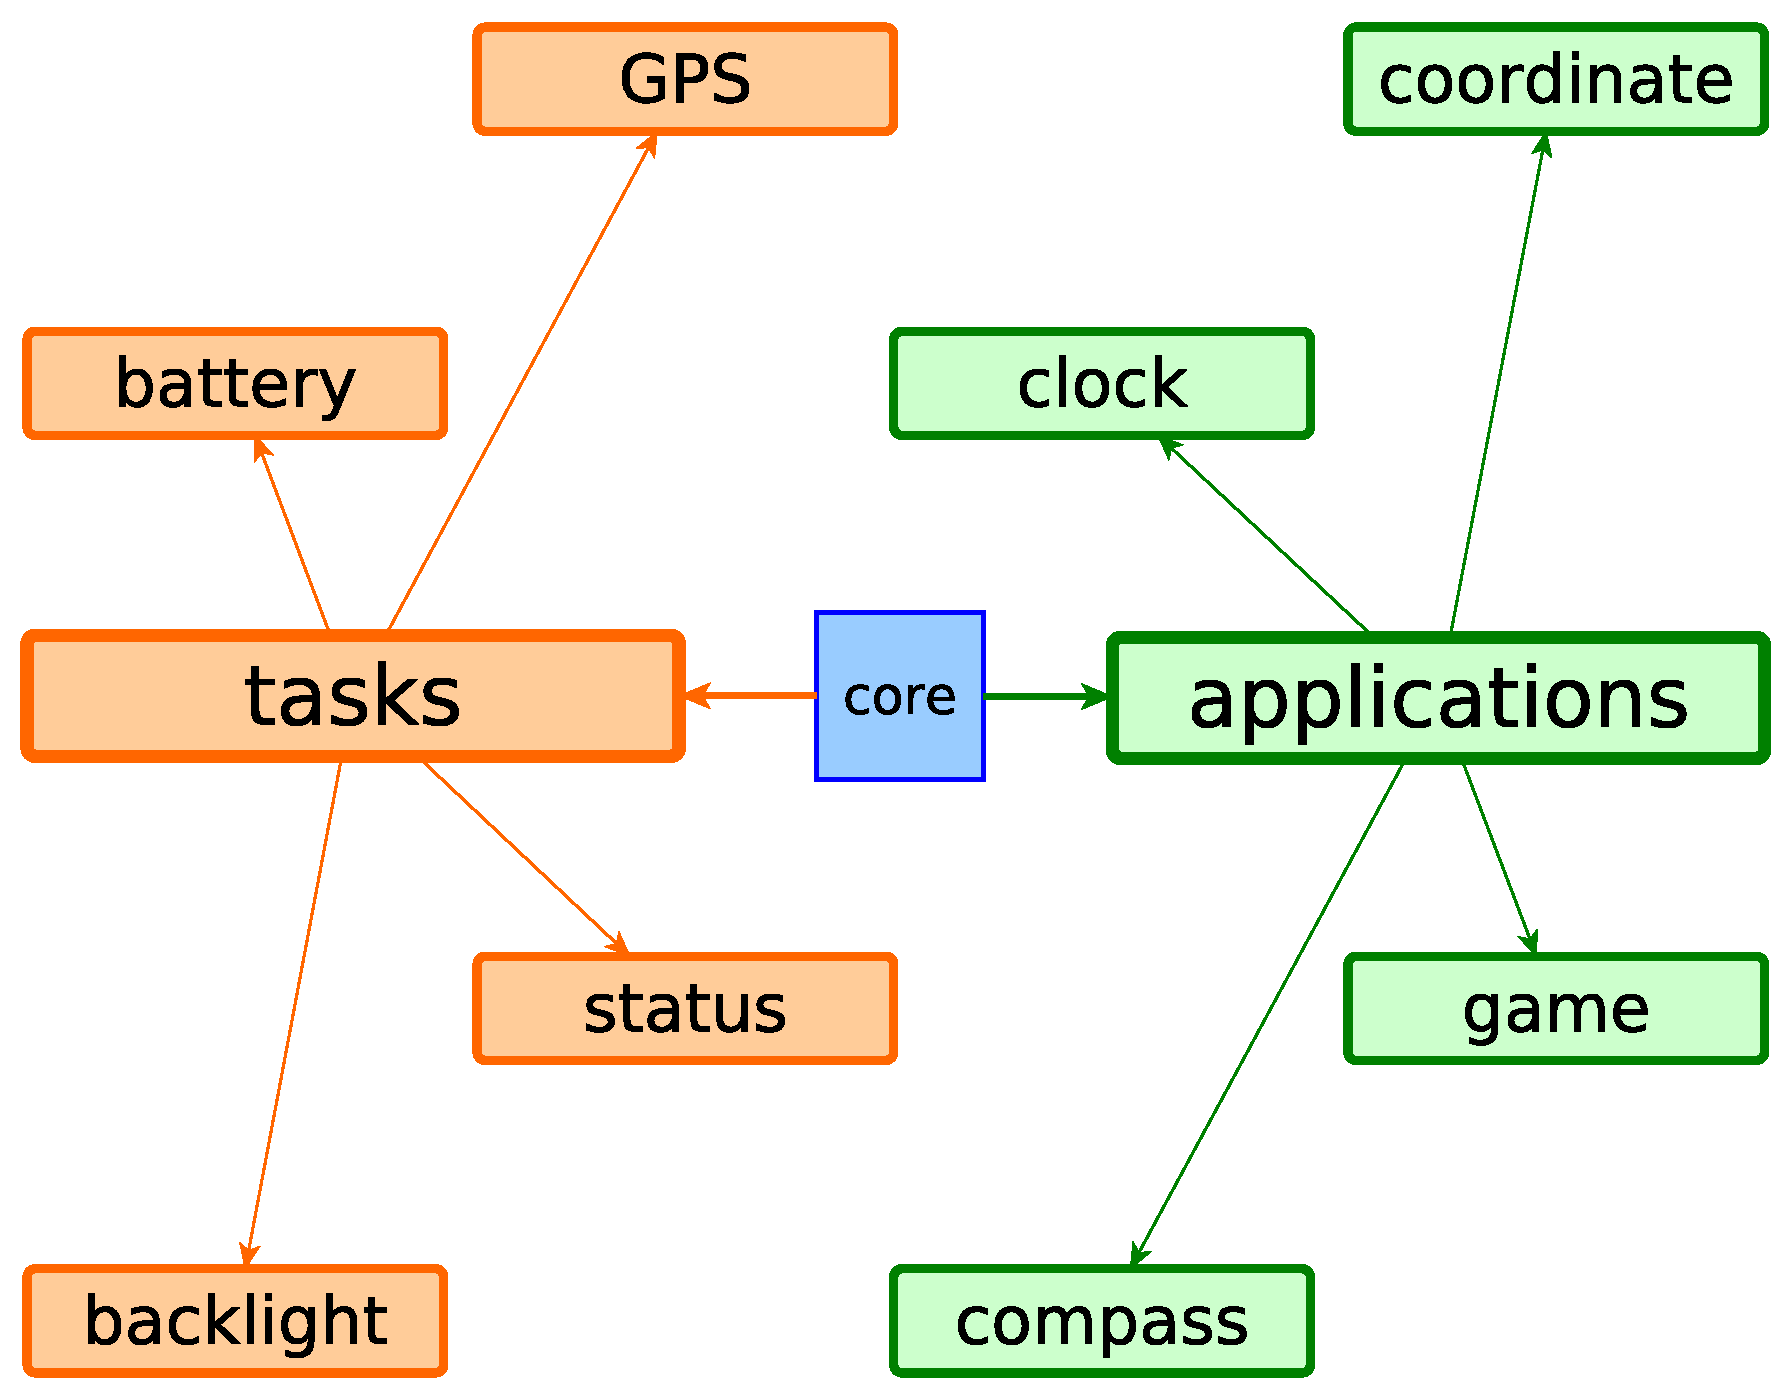
\includegraphics[height=7cm]{sw-app.eps}
  \end{center}

\end{frame}

%------------ FRAME --------------------------------------------------
\begin{frame}{Interface}
  \begin{center}
    \includegraphics[height=7.5cm]{fwatch-full-side-btn.eps}
  \end{center}
\end{frame}

%------------ FRAME --------------------------------------------------
\begin{frame}{Demo}
  \begin{center}

    \large Applications demonstration video

    %\begin{figure}[h!]
    %  \centering
    %  \movie[height=5cm, width = 5cm, autostart, once, showcontrols=true,
     %   borderwidth=1pt, poster]{Applications Demonstration}{../videos/fosdemlow.mp4}
    %\end{figure}
  \end{center}

\end{frame}

%------------ FRAME --------------------------------------------------
\begin{frame}{Documentation}
  \Large
  \begin{center}
      www.ohwr.org/projects/f-watch/wiki
  \end{center}
  \vskip 1cm
  \begin{itemize}
  \item how to configure your machine
    \vskip 7mm
  \item how to write applications
    \vskip 7mm
  \item details about the project
  \end{itemize}

\end{frame}


%#####################################################################
%############ SECTION ################################################
\section{Conclusions}

\begin{frame}{Development Summary}
  \Large
  \begin{columns}[T] % align columns
    \begin{column}{.55\textwidth}
      \begin{itemize}
      \item free PCB design
        \vskip 7mm
      \item free mechanic design
        \vskip 7mm
      \item free software
        \vskip 7mm
       \item free tools
         \vskip 7mm
       \item free time
      \end{itemize}
    \end{column}
    \hfill%
    \pause
    \begin{column}{.43\textwidth}
      \vskip 18mm
      \begin{center}
        \textbf{free} development \\
        for\\
        \textbf{free} products
      \end{center}
    \end{column}%
  \end{columns}
\end{frame}

%------------ FRAME --------------------------------------------------
\begin{frame}{Free Development Needs Free Tools}
  \begin{center}
    \alt<2> {
      \includegraphics[height=7.5cm]{fwatch-full-side-tool.eps}
    }{
      \includegraphics[height=7.5cm]{fwatch-full-side.eps}
    }
  \end{center}

\end{frame}

%------------ FRAME --------------------------------------------------
\begin{frame}{Easy to Make}
  \Large
  \begin{center}
    How difficult can it be? \\
    \vskip 1cm
    Competitive free tools \\
    \vskip 1cm
    Specialized company in 3D printing \\
    \vskip 1cm
    Specialized company in PCB manufacturing \\
    \vskip 1cm
    Easy to ship everywhere
 \end{center}

\end{frame}

%------------ FRAME --------------------------------------------------
\begin{frame}{Next Generation Free-Open Source}
  \Large
  \begin{center}
    Free products are real \\
    \vskip 1cm
    cars, robots, watches, bikes, houses, phones, ... \\
    \vskip 1cm
    3D Metal printers \\
  \end{center}

\end{frame}

%------------ FRAME --------------------------------------------------
\begin{frame}{What can it be?}
  \vskip -5mm
  \begin{columns}[T] % align columns
    \begin{column}{.48\textwidth}
      \begin{center}
        \includegraphics[height=3.5cm]{fwatch-para.eps} \\
        \vskip 5mm
        \includegraphics[height=3.5cm]{fwatch-tenn.eps}
      \end{center}
    \end{column}
    \hfill%
    \begin{column}{.48\textwidth}
      \begin{center}
        \includegraphics[height=3.5cm]{fwatch-bike.eps} \\
        \vskip 5mm
        \includegraphics[height=3.5cm]{fwatch-trek.eps}
      \end{center}
    \end{column}%
  \end{columns}

\end{frame}

%------------ FRAME --------------------------------------------------
\begin{frame}{Join Us}
  \Large
  \begin{center}
    \includegraphics[height=3.5cm]{fwatch-full-side.eps} \\
    \vskip 5mm
    Not a real product \\
    \vskip 5mm
    Make it a good example \\
    \vskip 5mm
    Join the project \\
  \end{center}

\end{frame}


\end{document}


